\chapter{Deep learning} \label{ch:deep-learning}

\indent \textit{Deep Learning} es un conjunto de métodos de aprendizaje que intentan modelar problemas con
arquitecturas complejas combinando diferentes transformaciones no lineales. Los pilares fundamentales son las redes
neuronales. Combinadas logran formar las \acrshort{dnn} (\textit{deep learning neural network}). \\
\indent Estas técnicas han logrado un avance significativo en los campos de procesamiento de sonidos y de imágenes,
éstos incluyen reconocimiento facial, reconocimiento del habla, visión computadorizada, entre otros.

\section{Redes neuronales}

\indent Una red neuronal artificial es una aplicación, no lineal respecto a su parámetros $\theta$ asociado a una
entrada $x$ y una salida $y = f(x,\theta)$. Por simplificación $y \in \mathbb{R}$ pero puede ser que $y$ sea
multidimensional, $\textbf{y} \in \mathbb{R}^n$. La red neuronal puede ser utilizada para regresión o clasificación.
En aprendizaje estadístico, como es usual, se estima un parámetros $\theta$ a partir de una muestra. Generalmente,
la función a minimizar no es convexa y resulta en minimizaciones locales. Existe un método muy eficiente para
computar el gradiente de una red neuronal. Éste llamado retropropagación del gradiente (\textit{backpropagation of
the gradient}), permite obtener una minimización local de un criterio cuadrático fácilmente.

\section{Perceptrón}

\indent Un perceptrón es una función $f_j$ de la entrada $\mathbf{x} = (x_1, ...,x_d)$ pesado por un vector
$\mathbf{w} = (w_{j,1}, ..., w_{j,d})$, completado por un sesgo $b_j$ y asociado a una función de activación $\phi$.

\begin{align}
  y_j = f_j(x) = \phi(<w_j,x> + b_j)
\end{align}

\subsection*{Funciones de activación}

\begin{itemize}
  \item Función de identidad:
  \begin{align}
    \phi(x) = x, \; -\infty < x < \infty
  \end{align}

  \item Función sigmoidea:
  \begin{align}
    \phi(x) = \frac{1}{1+e^{-x}}, \; -\infty < x < \infty
  \end{align}

  \item Función tangente hiperbólica:
  \begin{align}
    \phi(x) = \frac{e^{x}-e^{-x}}{e^{x}+e^{-x}} = \frac{e^{2x}-1}{e^{2x}+1}, \; -\infty < x < \infty
  \end{align}

  \item Función de umbral (\textit{hard-threshold}):
  \begin{align}
    \phi(x) = \mathbf{1}_{x \geq \beta}, \; -\infty < x < \infty
  \end{align}

  \item Función rectificadora lineal (\textit{rectified linear unit}):
  \begin{align}
    \phi(x) = \max(0,x), \; -\infty < x < \infty
  \end{align}
\end{itemize}

\indent En la Figura \ref{fig:neuron-schematic} se ilustra un esquemático de una neurona donde $\Sigma = <w_j,x> + b_j$.

\begin{figure}[H]
  \centering
  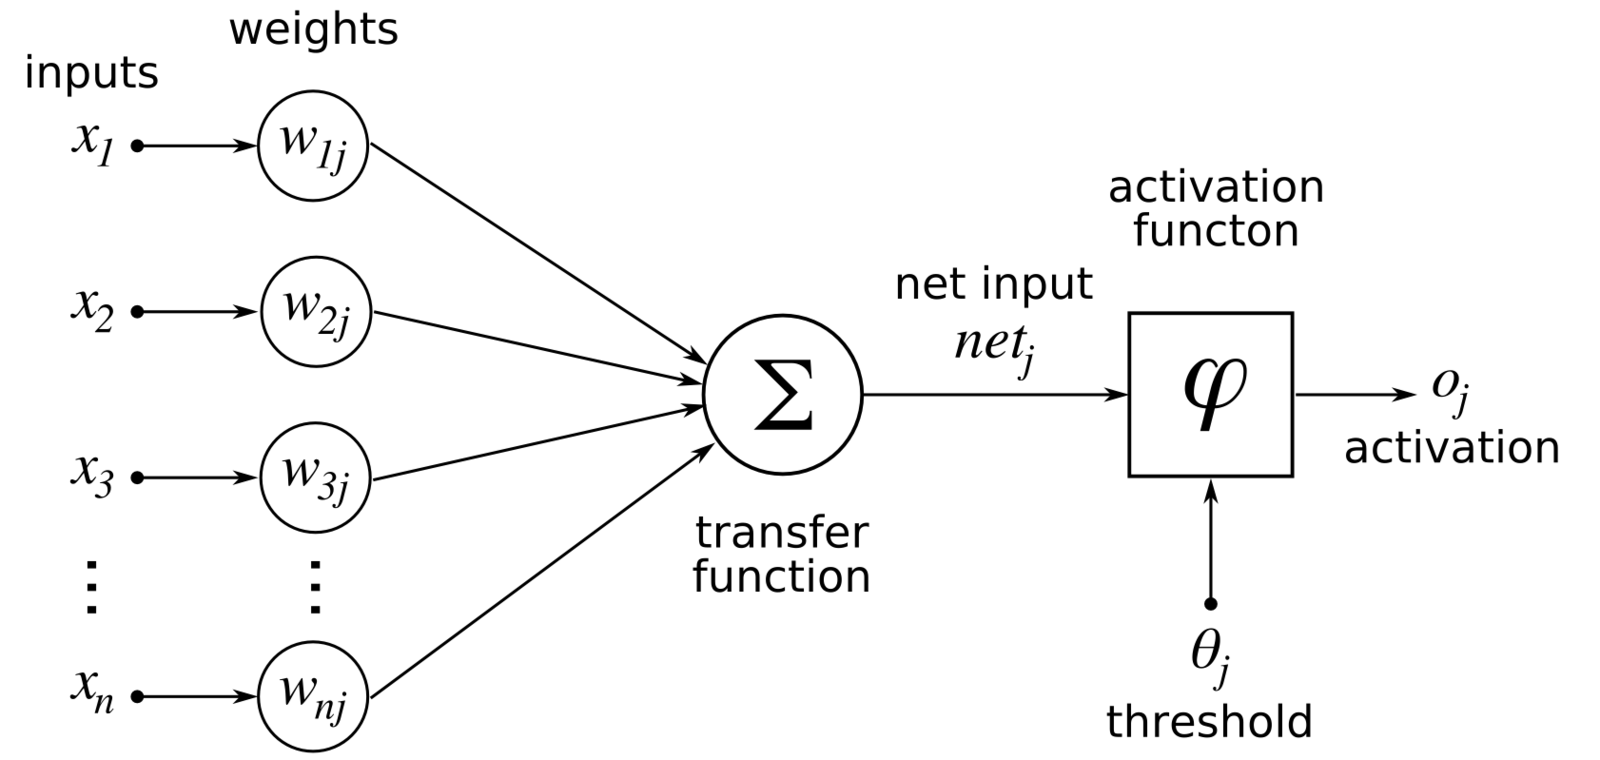
\includegraphics[scale=0.2]{sections/chapter-06/images/neuron-schematic.png}
  \caption[Esquemático de una neurona]{Esquemático de una neurona. Imagen obtenida de \href{https://commons
  .wikimedia.org/wiki/File:ArtificialNeuronModel_english.png}{Wikimedia Commons}.}
  \label{fig:neuron-schematic}
\end{figure}

\indent Históricamente, la función sigmoidea fue mayormente utilizada ya que es diferenciable y permite mantener los
valores entre [0,1]. Sin embargo, es problemática ya que su gradiente es muy cercano a cero cuando $|x|$ no se
encuentra cerca de 0.

\begin{figure}[H]
  \centering
  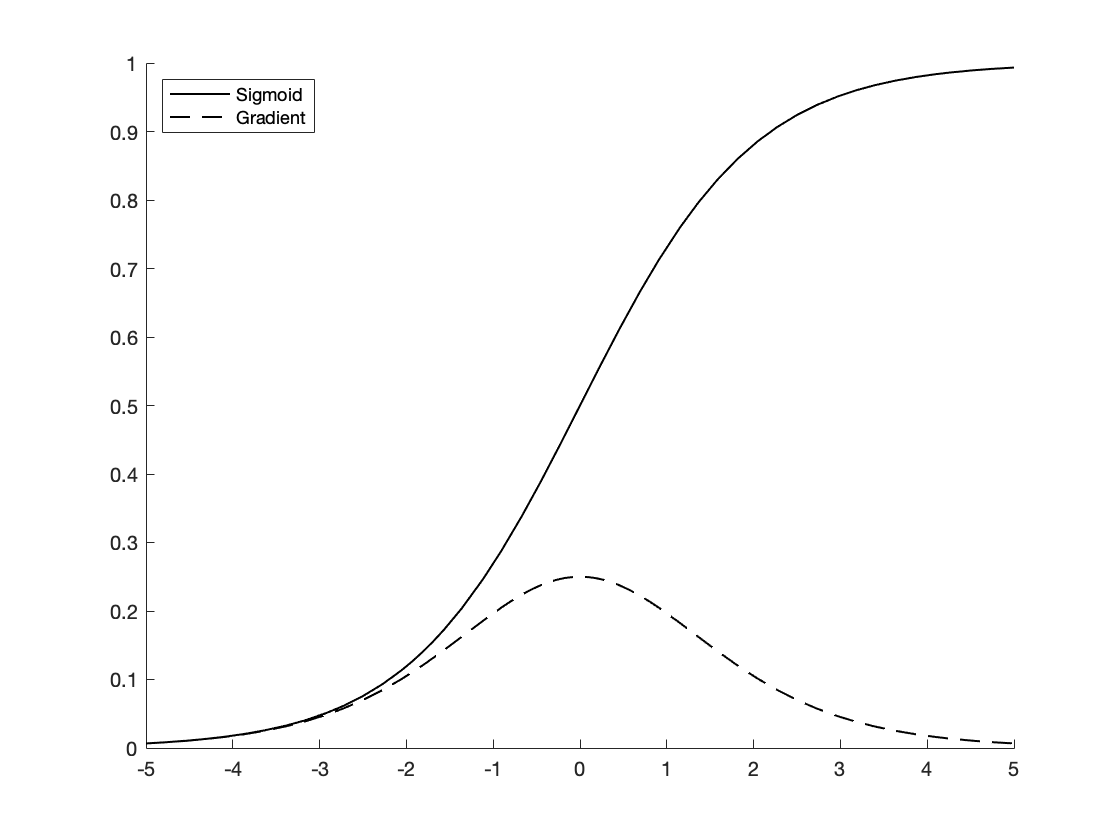
\includegraphics[scale=0.3]{sections/chapter-06/images/sigmoid.png}
  \caption[Función de activación sigmoidea.]{Función de activación sigmoidea.
  La línea sólida se muestra la función de activación y su derivada en línea punteada.}
  \label{fig:relu}
\end{figure}

\indent Es el caso de \textit{deep learning} que se utilizan múltiples capas de redes neuronales, lo cual trae
problemas
con el algoritmo de retropropagación para estimar parámetros. Éste es el por qué la función sigmoidea fue reemplazada
por la función \acrshort{relu} (\textit{Rectified Linear Unit}).

\begin{figure}[H]
  \centering
  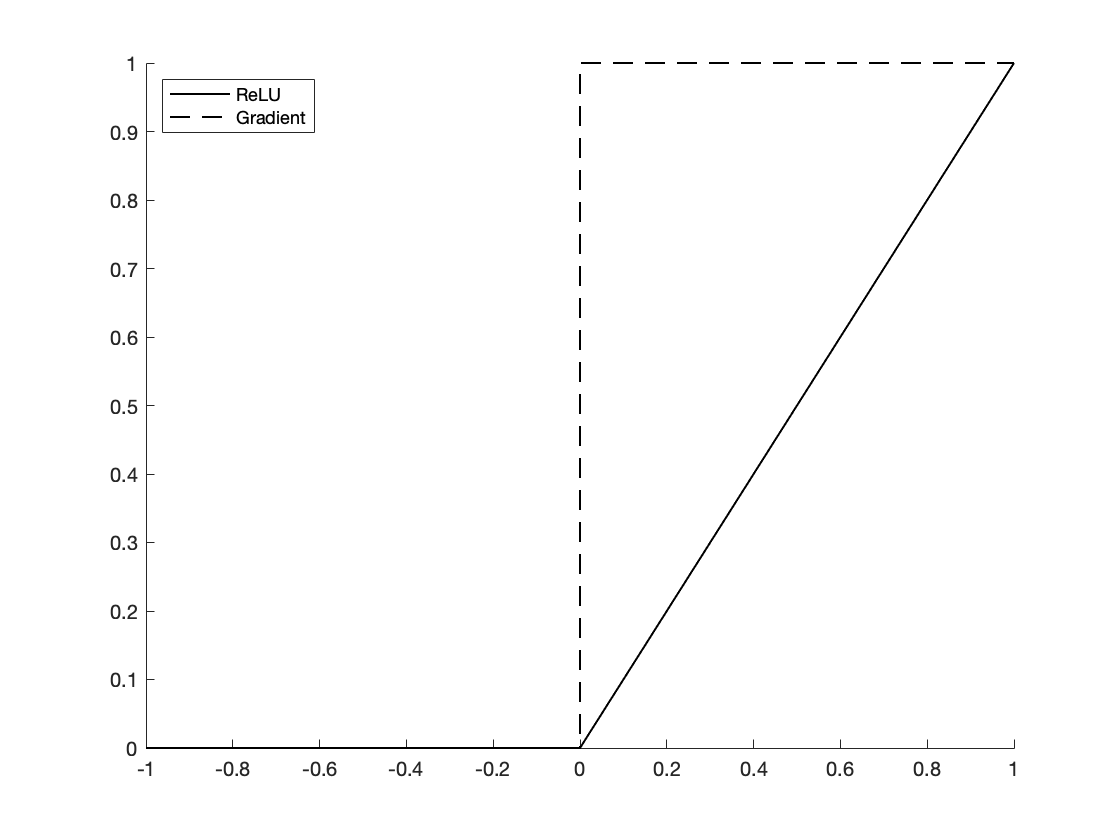
\includegraphics[scale=0.3]{sections/chapter-06/images/ReLU.png}
  \caption[Función de activación \acrshort{relu}.]{Función de activación \acrshort{relu}. La línea sólida se muestra
  la función de activación y su derivada en línea punteada.}
  \label{fig:sigmoid}
\end{figure}

\indent Esta función no es diferenciable en cero, pero en la práctica esto no es un problema dado que la
probabilidad de que una entrada sea igual a cero es casi nula. La función \acrshort{relu} también tiene la propiedad
de dispersión (\textit{sparcification}). Ella y su derivada son 0 para valores negativos, y no es posible obtener
información en estos casos, pero eso es recomendable agregar un pequeño sesgo para asegurar de que cada unidadad se
encuentre activa. Muchas variaciones de la función \acrshort{relu} consideran mantener a las unidades siempre
activas y que sus gradientes para valores negativos no sean 0.

\section{Perceptrón multicapa}

\indent Un perceptrón multicapa (o una red neuronal) es una estructura compuesta por varias capas, las cuales en la
literatura se las denomina capas ocultas (\textit{hidden layers}), compuestas por neuronas donde su salida son la
entrada de las neuronas de la siguiente capa. Más aún, la salida de una neurona puede ser la entrada de otra neurona
de la misma o anterior capa (es el caso de las redes neuronales recurrentes). En la última capa, denominada capa de
salida, es posible aplicar una función de activación distinta a las aplicadas en las capas intermedias dependiendo
del problema en cuestión: regresión o clasificación.

\begin{figure}[H]
  \centering
  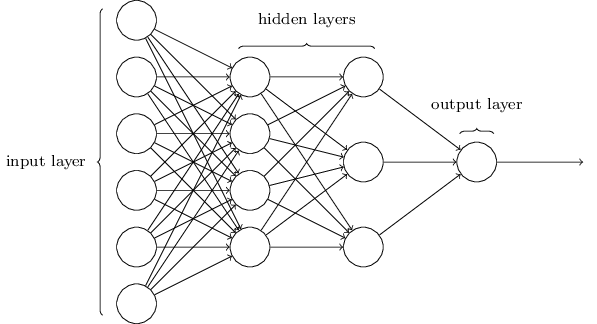
\includegraphics[scale=0.6]{sections/chapter-06/images/mlp-network.png}
  \caption[Perceptrón multicapa]{Perceptrón multicapa. Imagen obtenida del \href{https://github
  .com/rcassani/mlp-example}{repositorio de Raymundo Cassani}}
  \label{fig:mlp_net}
\end{figure}

\indent \acrshort{mlp} (Multilayer perceptron) tienen una arquitectura básica. Cada unidad o neurona de una capa se
conecta a todas las neuronas de la siguiente capa y no tienen conexión con las neuronas de la misma capa. Los
parámetros de la arquitectura son la cantidad de capas y el número de unidades por capa. Generalmente, como se ha
dicho antes, la función de activación es diferente a las otras intermedias. En el caso de clasificación binaria, la
salida genera una predicción de $\mathbb{P}(Y=1|X)$ ya que ese valor es [0,1], y la función de activación sigmoidea
es utilizada. Para un caso de clasificación multiclase (N es la cantidad de clases), la capa de salida se compone de
N neuronas, generando una predicción de $\mathbb{P}(Y=i|X)$, siendo $i=1,2,...,N$. Por supuesto, al ser
probabilidades, la suma de todas éstas deben sumar 1. \\
\indent La mayoría de las veces se usa la función multidimensional \textit{softmax}.

\begin{align}
  \mathrm{softmax}(z)_i = \frac{e^{z_i}}{\sum_j e^{z_j}}
\end{align}

\indent La formulación matemática para el perceptrón multicapa se define con $L$ capas intermedias.

\begin{enumerate}
  \item La capa de entrada (\textit{input layer}) se define para $k=0$.

  \begin{align*}
    h^{(0)}(\bm{x}) = \bm{x}
  \end{align*}

  \item Para las capas ocultas se define $k = 1,2,...,L$.

  \begin{align*}
    a^{(k)}(\bm{x}) &= \bm{b}^{(\bm{x})} + \mathbf{W}^{(k)}h^{(k-1)}(\mathbf{x}) \\
    h^{(k)}(\bm{x}) &= \phi(a^{(k)}(\bm{x}))
  \end{align*}

  \item Para $k = L+1$, la capa de salida (\textit{output layer}).

  \begin{align*}
    a^{(L+1)}(\bm{x}) &= b^{(L+1)} + \mathbf{W}^{(L+1)}h^{(L)}(\mathbf{x}) \\
    h^{(L+1)}(\bm{x}) &= \psi(a^{(L+1)}(\bm{x}))
  \end{align*}
\end{enumerate}

\indent Donde $\phi$ es la función de activación de las capas intermedias y $\psi$ la función de activación de la
capa de salida, en este caso la función \textit{softmax}. La matriz $\bm{W}^{(k)}$ tiene dimensiones  M $\times$ N,
donde M corresponde a la cantidad de neuronas en la capa $k$ y N a la cantidad de neuronas en la capa $k-1$.

\subsection*{Estimación de parámetros}

\indent Una vez definida la arquitectura de la red neuronal, los parámetros $\mathcal{D} = \{\bm{W}$, $\bm{b_j}\}$
deben ser estimados a partir de muestras. Como es común, estas estimaciones se obtienen a partir de la minimización
de lo que se cononce como función de costo (\textit{loss function}) \\
\indent Existen distintos tipos de funciones de costo. Éstas dependen del problema a resolver. 1) regresión:
\begin{itemize}
  \item Error cuadrático medio (\acrshort{mse})\footnote{La función de costo \acrshort{mse} se conoce también como:
  \item \textit{Quadratic Loss} o \textit{L2 loss}}
  \begin{align}
    \mathbf{MSE} = \frac{\sum_{i=1}^n (y_i - \hat{y}_i)^2}{n}
  \end{align}

  \item Error absoluto medio (\acrshort{mae})\footnote{Se conoce a la función de costo \acrshort{mae} como:
  \item \textit{L1 loss}}
  \begin{align}
    \mathbf{MAE} = \frac{\sum_{i=1}^n |y_i - \hat{y}_i|}{n}
  \end{align}

  \item Error de sesgo medio (\acrshort{mbe})
  \begin{align}
    \mathbf{MBE} = \frac{\sum_{i=1}^n (y_i - \hat{y}_i)}{n}
  \end{align}
\end{itemize}
2) Clasificación:

\begin{itemize}
  \item Costo bisagra (\textit{Hinge loss})
  \begin{align}
    \mathbf{L(\hat{y}_i,y)} = \sum_{j \neq y_i} \mathrm{max}(0, s_j-s_{y_i}+1)
  \end{align}

  \item Costo de entropía cruzada (\textit{Cross-entropy loss})
  \begin{align}
    \mathbf{L(\hat{y}_i,y)} = -(y_i \log(\hat{y}_i) + (1-y_i)\log(1-\hat{y}_i))
  \end{align}
\end{itemize}

\section{Inicialización}

\indent La información a la entrada debe normalizarse y los sesgos pueden ser inicializados en 0. No así, los pesos
ya que en el caso de la función de activación $tanh$, su derivada en 0 es 0, el cual es un punto de silla. Tampoco
pueden ser inicializados con los mismos valores, de lo contrario todas las neuronas tendrían el mismo comportamiento
. Usualmente estos valores se inicializan de form aleatoria: $W_{i,j}^{(k)} \sim \mathcal{U}[-c,c]$, i.i.d con
$c=\frac{\sqrt{6}}{N_k+N_{k-1}}$ donde $N_k$ es el tamaño de la capa k. También se suele inicializar los pesos con
una distribución normal, $W_{i,j}^{(k)} \sim \mathcal{N}(0,0.01)$.

\section{Hiperparámetros}

\indent Existen una variadad extensa de algoritmos para minimizar las funciones de costo y todos estos poseen
hiperparámetros que deben ser calibrados. Éstos tienen un impacto importante en la convergencia de los mismos. Una
herramienta básica en todos estos algoritmos es lo que se conoce como \acrshort{sgd} (\textit{Stochastic Gradient
Descent}). Es la más simple.

\begin{align}
  \theta_i^{new} = \theta_i^{old}-\epsilon \frac{\partial L}{\partial \theta_i}(\theta_i^{old})
\end{align}

\indent Donde $\epsilon$ es lo que se conoce como tasa de aprendizaje (\textit{learning rate}). Si es muy pequeño,
la convergencia es muy lenta y puede quedar bloqueada en un mínimo local. Si es muy grande, la convergencia puede
oscilar alrededor de un óptimo sin estabilizarse y converger. Es recomendable comenzar con un $\epsilon$ grande e ir
iterando. \\
\indent El algoritmo \acrshort{sgd} consiste en computar el gradiente. Para ello se considera la técnica de
aprendizaje por lotes (\textit{batch learning}), en el que en cada paso $m$ muestras son elegidas al azar y la media
de esas $m$ muestras se utilizara para actualizar los parámetros. Luego, otro concepto es lo que se denomina como
\textit{epoch}, proveniente del inglés. Se define \textit{epoch} al paso de todo el set de entrenamiento por la red
neuronal una vez y se encuentra íntimamente relacionado con el tamaño del lote (\textit{batch size}). Es decir, si
el tamaño es 1/100, significa que un \textit{epoch} contiene 100 batches. La cantidad de \textit{epochs} es a su vez
un hiperparámetro a calibrar. \\
\indent Existen técnicas para detener la estimación, conocido como parada temprana (\textit{early stopping}) y
consiste en considerar un set de validación en el cual se detiene la estimación cuando la función de costo de este
set de datos deja de decrecer. El método de aprendizaje por lotes es utilizado por motivos computacionales. El
algoritmo de retropropagación mencionado antes necesita guardar todos los valores intermedios y para grandes set de
datos como han de ser imágenes resulta prácticamente inviable. Como se ha visto, el tamaño del lote es un
hiperparámetro el cual debe ser definido previamente y cuanto más pequeño mejores resultan las generalizaciones de
las estimaciones. En el caso de que sea igual a 1, se conoce como gradiente online descendente (\textit{on-line
gradient descent}). \\
\indent Una técnica que hoy en día se utiliza en su mayoría para mitigar el problema de la generalización de estos
métodos es la técnica de abandono (\textit{drop-out}). Consiste en definir una probabilidad $p$, la cual resulta en
otro hiperparámetro, algunas unidades de la red se fijan a 0. Tradicionalmente se utiliza 0.5 para las capas
intermedias y 0.2 para la capa de entrada. Computacionalmente este método no es costoso dado que es cambiar los
pesos de algunas unidades a 0.

% \section{Redes neuronales convolucionales}

% \indent Existen problemas, donde los \acrshort{mlp} no resuelven determinadas cuestiones y no se adaptan. Los perceptrones multicapa tienene como entrada vectores, los cuales en los casos que la información proviene de imágenes, deberían transformarse las imágenes en vectores perdiendo la forma de noción espacial que proveen éstas. Las redes convolucionales actuan directamente sobre matrices o tensores con tres canales \acrshort{rgb}. Actualmente las \acrshort{cnn}, se utilizan para clasificación, segmentación, reconocimiento de objetos y reconocimiento facial.

% \subsection{Capas en una red convolucional}

% \indent Una \acrshort{cnn} puede estar compuesta por distintas capas intermedias: capas convolucionales, \textit{pooling layers}, \textit{fully conected layers}.

% \subsection{Capa convolucional}

% \indent Una convolución discreta entre dos funciones $f$ y $g$ está definido por

% \begin{align}
%     (f * g)(x) = \sum_t f(t)g(x+t)
% \end{align}

% \indent Para señales bidimensionales como han de ser imágenes, se considera la convolución 2-D.

% \begin{align}
%     (K * I)(i,) = \sum_t K(m,n)I(i+n,j+m)
% \end{align}

% \indent El principio de esta herramienta matemática es desplazar una función K sobre la imagen, de tal manera que en cada posición de la imagen un valor es computado. La función K es un filtro que se desplaza una cantidad de pixeles, este es el paso (\textit{stride}) de la capa. También se utiliza rellenar con ceros (\textit{zero padding}) para mantener las dimensiones de la entrada y salida iguales. Asumiendo que se aplican $C_0$ filtros, cada uno de tamaño $k \times k$ en una imagen. Si el tamaño de la imagen es o tensor es de $W_i \times H_i \times C_i$, ancho, altura y canales respectivamente. El volúmen de la salida es $W_0 \times H_0 \times C_0$ y,

% \begin{align*}
%     W_0 &= \frac{W_i - k + 2p}{s} + 1 \\
%     H_0 &= \frac{H_i - k + 2p}{s} + 1
% \end{align*}

% Donde $p$ es el rellenado (\textit{padding}).

% \begin{figure}[H]
%     \centering
%     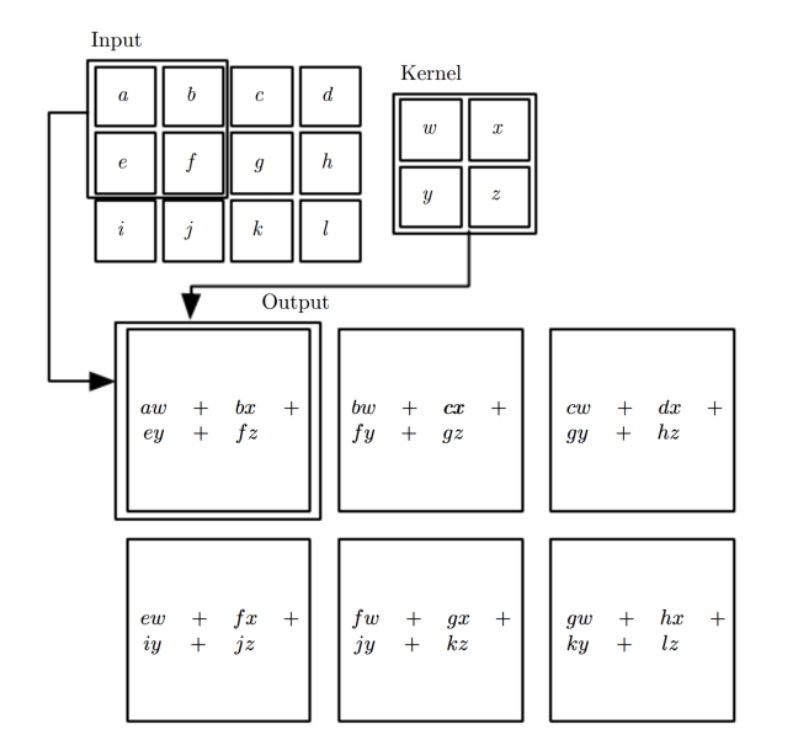
\includegraphics[scale=0.75]{sections/chapter-06/images/2-d-convolution-example.png}
%     \caption[Convolución 2D]{Convolución 2D. Imagen extraída de \href{https://www.deeplearningbook.org}{\textit{"Deep Learning Book"}}}
%     \label{fig:2d-convolution-example}
% \end{figure}

% \indent En el ejemplo de la Figura \ref{fig:2d-convolution-example} la imagen, $I \in \mathbb{R}^{3\times4}$ y el filtro, $K \in \mathbb{R}^{2 \times 2}$ con un $s = 1$ y $p = 0$, se obtiene una salida de $2 \times 3 \times 1$ ($C_0$ es 1). \\
% \indent Las operaciones de convolución son combinadas con una función de activación $\phi$ (generalmente la función \acrshort{relu}). Si se considera un filtro de $k \times k$, si $\mathbf{x}$ es una porción $k \times k $ de la imagen, la activación se obtiene tras deslizar una ventana de $k \times k$ y computando $z(\bm{x})=\phi(\bm{K} \cdot \bm{x}+\bm{b})$, donde $\bm{b}$ es el sesgo.

% \subsection{Pooling layer}

% \indent Las \acrshort{cnn} tiene capas que permiten reducir las dimensiones, también referido como submuestreo, tomando la media o el máximo en porciones de la imagen (\textit{mean-pooling} o \textit{max-pooling}). A su vez, este tipo de capas tienen, al igual que las capas convolucionales, un paso o stride. Otra propiedad, es la de hacer la red menos sensible a pequeñas transiciones de la imagen de entrada.

% \subsection{Fully-connected layers}

% \indent Luego de haber aplicado varias capas convolucionales, las \acrshort{cnn} terminan con una \textit{fully-connected layer}. El tensor a la salida de estas capas son transformadas en vectores como entradas a perceptrones.

\section{Redes neuronales recurrentes} \label{sec:rnn}

\indent A fin de inferir data secuencial, tal como texto o señales en el tiempo, aparecen las redes neuronales
recurrentes. La forma más simple de una red neuronal recurrente tiene múltiples copias de la misma red, cada una
pasando información a su sucesora. La primer red neuronal recurrente, era una \acrshort{mlp} con un bucle hacia si
misma. Definiendo $x(t)$, $\hat{y}(t)$, $\hat{z}(t)$ como la entrada, la salida y la capa intermedia en tiempo $t$
respectivamente.

\begin{align*}
  \hat{y}^{(k)}(t) &= \sum_{i=1}^{I} \bm{W}_i^{(k)} \hat{z}_i(t) + \bm{b}^{(k)} \\
  \hat{z}_i(t) &= \sigma\left(\sum_{j=1}^J w_{i,j}x_j(t) + \sum_{l=1}^I \Tilde{w}_{i,l} \hat{z}_l(t-1) + b_i \right)
\end{align*}

\indent Donde $\sigma$ es la función de activación. Las neuronas que son retroalimentadas asimismas, se denominan
\textit{context units} o unidades contextuales. Estos modelos y variaciones del mismo se han utilizado en el campo
del análisis lingüístico. Aunque, nuevas arquitecturas se han desarrollado para abordar estos problemas.

\subsection*{Long Short-Term Memory}

\indent Las RNN han sido exitosas en varias aplicaciones como han de ser reconocimiento del habla, traducción, entre
otros. Este éxito se debe a la eficiencia de las redes \acrshort{lstm}, que es una especie de red recurrente. Las
redes \acrshort{lstm} fueron introducidas por Hochreiter y Schmidhuber (1997) \cite{pp:hochreiter-schmidhuber} y
fueron creadas con el propósito de aprender dependencias a largo plazo. Una celda \acrshort{lstm} comprende, en un
instante $t$, un estado $C_t$ y una salida $h_t$. Como entrada, la celda requiere $x_t$, $C_{t-1}$, $h_{t-1}$.
Dentro de la celda, existen compuertas o \textit{gates} que permiten, o no, el paso de información. Este
comportamiento está dado por el siguiente conjunto de ecuaciones.

\begin{itemize}
  \item \textit{Update gate H}
  \begin{align}
    u_t = \sigma(\bm{W}^u h_{t-1} + \bm{I}^u x_t + b^u)
  \end{align}

  \item \textit{Forget gate H}
  \begin{align}
    f_t = \sigma(\bm{W}^f h_{t-1} + \bm{I}^f x_t + b^f)
  \end{align}

  \item \textit{Cell candidate H}
  \begin{align}
    \Tilde{C}_t = \mathrm{tanh}(\bm{W}^c h_{t-1} + \bm{I}^c x_t + b^c)
  \end{align}

  \item \textit{Cell output H}
  \begin{align}
    C_t = f_t \odot C_{t-1} + u_t \odot \Tilde{C}_t
  \end{align}

  \item \textit{Output gate H}
  \begin{align}
    o_t = \sigma(\bm{W}^o h_{t-1} + \bm{I}^o x_t + b^o)
  \end{align}

  \item \textit{Hidden output H}
  \begin{align}
    h_t = o_t \odot \mathrm{tanh}(C_t)
  \end{align}

  \item \textit{Output K}
  \begin{align}
    y_t = \mathrm{softmax}(\bm{W} \cdot h_t + b)
  \end{align}

  \item \textit{Recurrent weights H $\times$ H}
  \begin{align}
    \bm{W}^u, \bm{W}^f, \bm{W}^c, \bm{W}^o
  \end{align}

  \item \textit{Input weights N $\times$ H}
  \begin{align}
    \bm{I}^u, \bm{I}^f, \bm{I}^c, \bm{I}^o
  \end{align}

  \item \textit{Biases}
  \begin{align}
    b^u, b^f, b^c, b^o
  \end{align}
\end{itemize}

\indent La Figura \ref{fig:lstm-schematic} refleja la diferencia entre una celda RNN tradicional y una celda
\acrshort{lstm}. Una celda RNN contiene sólo una capa. En cambio, la celda \acrshort{lstm} contiene 4 capas dadas
por los bloques amarillos, interactuando entre ellas como se describen en las ecuaciones anteriores.

\begin{figure}[H]
  \centering
  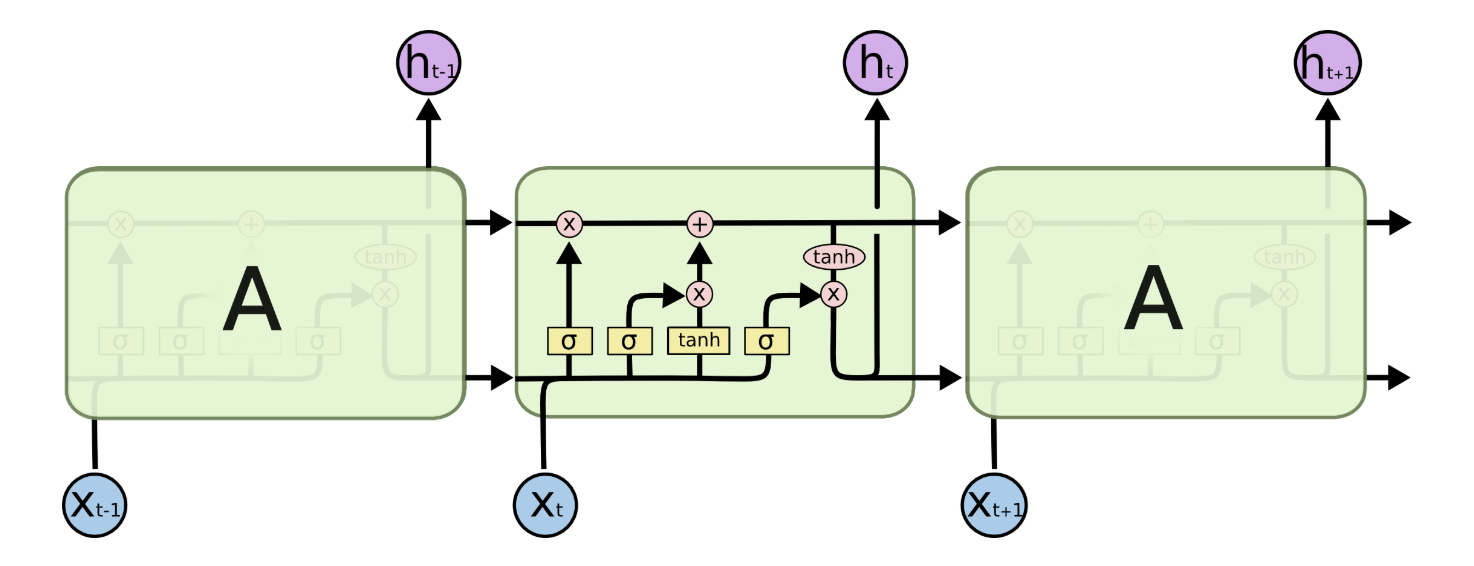
\includegraphics[scale=0.5]{sections/chapter-06/images/lstm-schematic.png}
  \caption[Diagrama de una red \acrshort{lstm}]{Diagrama de una red \acrshort{lstm}. Imagen extraída de
  \href{http://colah.github.io/posts/2015-08-Understanding-\acrshort{lstm}s/}{\textit{"Understanding \acrshort{lstm}
  Networks"}}}
  \label{fig:lstm-schematic}
\end{figure}

\indent Las redes \acrshort{lstm} son las elegidas en este trabajo. La particularidad de estas redes, como se ha
mencionado anteriormente, es la eficiencia para los problemas de señales en el tiempo.

\section{Sobre-entrenamiento}

\indent Estadísticamente hablando sobre-entrenamiento (\textit{overfitting}) se produce cuando un modelo corresponde
exactamente al conjunto de datos al que utiliza para estimar sus parámetros. Esto produce que predecir observaciones
futuras sea confiable. Un modelo sobre-entrenado generalmente tiene muchos más parámetros de los que se pueden
justificar con los datos de entrenamiento. Esencialmente, un modelo de estas características tiene por aprender
información descorrelacionada con los datos, por ejemplo ruido, como si fuese información representativa del modelo. \\
\indent Existe otro fenómeno de los modelos estadísticos, denominado sub-entrenamiento (\textit{underfitting}), que
contrario al sobre-entrenamiento ocurre cuando el modelo no es capaz de capturar la estructura de los datos, y sus
parámetros quedan en un estado indefinido.

\subsection*{Validación cruzada} \label{subsec:cross-validation}

\indent Antes de entrar en detalle en la extracción de los atributos tiempo-frecuencia, es necesario definir el
método de entrenamiento elegido en este trabajo. \\
\indent Validación cruzada (\textit{cross-validation}) es un método de validación de un modelo que analiza los
resultados estadísticos tal que éstos se encuentren los más generalizado a cualquier set de datos.
Es comúnmente usado donde el objetivo es la predicción, y se quiere saber cuán exacto y preciso el modelo predictivo
es en la práctica.
En un problema de predicción, se define un set de datos de entrenamiento y otro conjunto de datos de
evaluación. El primero, es un conjunto de datos en el cual el modelo predictivo estimará sus parámetros para luego
predecir datos que no hayan sido visto nunca.
Aquí es cuando entra el conjunto de datos de evaluación, que va a ser visto por primera vez por el modelo. Este
método tiene como objetivo solucionar el problema de sobre-entrenamiento. \\
\indent Existen varias técnicas dentro de validación cruzada. En este trabajo se hará hincapié en el denominado
\textit{K-Folds}.
Éste consiste en dividir el set completo de datos en $K$ grupos (generalmente es común utilizar $K = 10$).
El entrenamiento por ende se realizará $K$ veces, eligiendo en cada iteración un grupo de evaluación que no haya sido
elegido previamente. El resto de los grupos se utilizarán como entrenamiento.
De esta manera se computarán todas las métricas elegidas, $K$ veces y se computará la media, y el desvío de cada una
de ellas.

\section{Métricas} \label{sec:metrics}

\indent Determinar métricas de error es fundamental a la hora de evaluar cuáles son los próximos pasos a seguir. \\
\indent Hay que tener en cuenta que en algunas aplicaciones es prácticamente imposible obtener un error nulo.
El error de Bayes define el mínimo error que se puede esperar alcanzar, aún obteniendo una cantidad infinita de datos y
recuperando la verdadera función de distribución. Este se debe a que los atributos pueden no contener toda la
información que se necesita para explicar la variable de salida o porque el sistema a analizar puede ser
intrínsecamente estocástico. En la práctica uno siempre va a estar limitad por una cantidad finita de datos. \\
\indent La cantidad de datos puede estar limitada por varios motivos.
Por ejemplo, cuando el objetivo es construir un producto o servicio comercializable, uno puede siempre conseguir más
datos pero es necesario evaluar cuál es el costo del mismo comparado a tratar de reducir el error. La recolección de
datos implica tiempo, dinero y esfuerzo humano.
Un ejemplo típico del esfuerzo humano, cuando se necesita conseguir datos de un paciente clínico por medio
de técnicas invasivas.
En el ámbito académico o de investigación, cuando el objetivo es responder una pregunta científica sobre qué
algoritmo tiene mejor rendimiento en base a un estándar (\textit{benchmark}), no es posible agregar más datos. \\
\indent En muchas aplicaciones la exactitud (\textit{accuracy}) alcanza para definir el rendimiento de los
algoritmos.
Sin embargo, en muchas ocasiones esto no es así.
Es el ejemplo de la detección de una rara enfermedad, en la que una persona en un millón padecen esta enfermedad.
Por ende, una forma fácil de alcanzar $99.9999\%$ de exactitud es simplemente diciéndole al equipo que reporte que en
todos los casos la enfermedad se encuentra ausente.
Claramente, esta métrica no es útil y una forma de resolver esto es utilizando otras métricas como son la precisión
y sensibilidad (\textit{recall}).
La precisión se define como la cantidad de detecciones que el algoritmo definió
como correctas y sensibilidad es la cantidad de eventos verdaderos que fueron detectados. Un detector que dice que
nadie tiene esta enfermedad, tiene $100\%$ de precisión pero 0 sensibilidad. Un detector que dice que todos tienen
la enfermedad, tiene $100\%$ de sensibilidad pero precisión igual a la cantidad de las personas que sí la tienen, $0
.0001\%$ en este ejemplo. En muchas aplicaciones, es bueno resumir esta información en una sola métrica. Esta
métrica se conoce como métrica F$_1$.

\indent Otra opción es reportar el área bajo la curva P-R, donde en el eje de abscisas se encuentra R y en el eje de
ordenadas, P. \\
\indent Muchas otras métricas son posibles. En distintas aplicaciones especializadas, existen métricas
característica de ese campo. \\
\indent Una manera de mostrar rendimiento de un algoritmo de estimación, es por medio de la matriz de confusión.
Esta matriz representa en sus columnas las clases verdaderas y las filas contienen a las clases estimadas. Esta
matriz resume distintas métricas, de las cuales es posible obtener resultados. Estas métricas se especifican en función
de los falsos positivos (FP), falsos negativos (FN), verdaderos positivos (TP) y verdaderos negativos (TN).

\begin{itemize}
  \item Sensibilidad
  \begin{align}
    \acrshort{tpv} = \frac{\acrshort{tp}}{\acrshort{tp}+\acrshort{fn}}
  \end{align}

  \item Especificidad
  \begin{align}
    \acrshort{tnr} = \frac{\acrshort{tn}}{\acrshort{tn}+\acrshort{fp}}
  \end{align}

  \item Precisión
  \begin{align}
    \acrshort{ppv} = \frac{\acrshort{tp}}{\acrshort{tp}+\acrshort{fp}}
  \end{align}

  \item Valor Predictivo Negativo
  \begin{align}
    \acrshort{npv} = \frac{\acrshort{tn}}{\acrshort{tn}+\acrshort{fn}}
  \end{align}

  \item Tasa de error
  \begin{align}
    \acrshort{fnr} = \frac{\acrshort{fn}}{\acrshort{fn}+\acrshort{tp}}
  \end{align}

  \item Tasa de falsos positivos
  \begin{align}
    \acrshort{fpr} = \frac{\acrshort{fp}}{\acrshort{fp}+\acrshort{tn}}
  \end{align}

  \item Tasa de descubrimiento
  \begin{align}
    \acrshort{fdr} = \frac{\acrshort{fp}}{\acrshort{fp}+\acrshort{tp}}
  \end{align}

  \item Tasa de omisión
  \begin{align}
    \acrshort{for} = \frac{\acrshort{fn}}{\acrshort{fn}+\acrshort{tn}}
  \end{align}

  \item Exctitud
  \begin{align}
    \acrshort{acc} = \frac{\acrshort{tp}+\acrshort{tn}}{\acrshort{tp}+\acrshort{tn}+\acrshort{fn}+\acrshort{fp}}
  \end{align}

  \item Puntaje F$_1$
  \begin{align}
    F_1 = \frac{2\acrshort{tp}}{2\acrshort{tp}+\acrshort{fp}+\acrshort{fn}}
  \end{align}
\end{itemize}

\indent Las métricas que aquí se trabajarán son exactitud ($ACC$), precisión ($P_+$), sensibilidad ($Se$) y $F_1$.
Los motivos de esta decisión es la naturaleza de la aplicación y por comparación de desempeño con otros trabajos
publicados. \\
\indent \acrshort{tp} define a los verdaderos positivos y \acrshort{tn} a los verdaderos negativos. En base a estos
dos parámetros se pueden calcular todas las métricas mencionadas. Por otro lado, cabe destacar que dependiendo de la
cantidad de clases que el problema posea, es necesario computar \acrshort{tp} y \acrshort{tn} para cada una de ellas.
